%%%%%%%%%%%%%%%%%%%%%%%%%%%%%%%%%%%%%
%%%%% PHYS305 Assignment 10
%%%%% Zachary Martin
%%%%% 16 April 2019
%%%%%%%%%%%%%%%%%%%%%%%%%%%%%%%%%%%%%

\documentclass[aps,prl,twocolumn,superscriptaddress]{revtex4-1}

\usepackage{graphicx}  % this is the up-to-date package for all figures
\graphicspath{{Pictures/}} 	% Set Graphics Path
\usepackage{siunitx} % Scientific Notation and Units
\sisetup{separate-uncertainty}
\DeclareSIUnit\mph{mph}
\usepackage{amsmath, amssymb, gensymb, mathtools, bm, bigints} 	% Mathematical Tools
\usepackage{verbatim}  % for the comment environment
\usepackage{color}
% \usepackage{arydshln} % Dashed lines in table

% For inserting code snippets
\usepackage{listings}
\usepackage{xcolor}
\lstset { %
    language=C++,
    backgroundcolor=\color{black!5}, % set backgroundcolor
    basicstyle=\footnotesize,% basic font setting
}

% Shortcut Commands
\newcommand{\paren}[1]{\left( #1 \right)} 	% Parentheses for complicated expressions
\newcommand{\bparen}[1]{\left[ #1 \right]}	% Bracket parentheses for complicated expressions
\newcommand{\cmod}[1]{\left| #1 \right|}	% Mod or Absolute value

\bibliographystyle{apsrev}

% these are some custom control of the page size and margins
% \topmargin= 0.2in  % these 1st two may be needed for some computers
\textheight=9in
\textwidth=6.5in
% these next two lines give us centered text
\oddsidemargin=0cm
\evensidemargin=0cm

%\begin{figure}[htbp]
%  	\begin{center}
% 		\includegraphics[scale=0.3]{.png}
%  		\caption{}
%  		\label{gr:}
% 	\end{center}
%\end{figure}

\begin{document}

% Title Contents
\title{PHYS 305 Assignment 10: Simulating the Earth, the Moon, and Apollo 13.}
\author{Zachary Martin}
\affiliation{University of Hawaii at Manoa}
\date{16 April 2019}

\begin{abstract}
We examine efforts taken to launch a spacecraft to the moon by simulating the Earth-Moon system and plotting different trajectories on a spacecraft based on trial and error. We come to appreciate the incredible effort by NASA and the Apollo program for successfully bring this feat to fruition. The difficulties of such a project are realized through the dramatic changes of a trajectory from subtle changes in launch conditions. Here, we have simplified the model to focus only on the trip in space, and assumed circular orbits of the moon and Earth around the barycenter. Even then, we find it incredibly difficult to find a trajectory to hit the moon, especially at a low velocity. Our attempts to orbit the moon were not successful, but round trip trajectories from the moon and back to Earth were found from adjusting the hit trajectories.
\end{abstract}

\maketitle

\section{Introduction and Overview}
Mankind began to voyage out into space in the late 1950's. NASA developed the Apollo program in an effort to get humans on the moon. It wasn't until Apollo 11 that successfully got the first humans, Neil Armstrong and Edwin "Buzz" Aldrin, to step foot on the moon in 1969 \cite{space}. While it seems like a miraculous feat of human effort, it was rigorous and carefully calculated. To reach the moon took an incredible amount of precise calculations, importantly so for the sake of lives. 

On April 1970, Apollo 13 was launched to the moon, as NASA's third trip to carry humans to the moon. Unfortunately, a faulty oxygen tank was installed onto the spacecraft, which during flight had exploded \cite{apollo}. In order to save the astronauts aboard, their trajectory had to loop around the moon and return safely to Earth. The calculations were incredibly important here, and were they not done correctly, Apollo 13 may not had come back. We thus examine the efforts of space travel to the moon using computational methods. 

\section{Set Up \& Relevant Equations}
To simplify our space travel problem, we consider our Apollo spacecraft to already be in a parked orbit $\SI{175}{\km}$ above the surface of the Earth. We also assume an instantaneous launch, thus ignoring the need for thrust. Then, the most important force acting on our bodies, Earth, the moon, and Apollo, is gravity:
\begin{equation}
\vec{F_{1,2}} = - \vec{F_{2,1}} = \frac{GMm}{\cmod{\vec{r_1} - \vec{r_2}}^3} \paren{\vec{r_1} - \vec{r_2}} ~.  \label{eq:grav}
\end{equation}
This is an attractive force between two bodies, parallel to the line connecting them. This equation from Newton's law of gravitation \cite{lab} conserves the vector property of the gravitational force. We will ignore the gravitational pull of Apollo, as the mass is negligible compared to the mass of the moon and Earth.

Before we introduce our spacecraft into the cosmos, we wish first to simulate the orbit of the moon around the Earth. We will do so in the barycentric (center of mass) frame, using the distances
\begin{equation}
r_1 = \frac{m_2}{m_1 + m_2} D_{1,2} ~. \label{eq:cmdist}
\end{equation}
The moon and Earth have an established velocity that we need to give in order to keep the orbit as we want. In this case, we will assume a circular orbit for both bodies around the barycenter. Such a case yields a necessary tangential velocity of
\begin{equation}
v_{\text{orb}} = \frac{2\pi r}{T} ~, \label{eq:orbvel}
\end{equation}
where $T$ is the common orbital period given by \cite{phys}
\begin{equation}
T = 2\pi \sqrt{\frac{r^3}{GM}} ~.  \label{eq:period}
\end{equation}
The energy contained in the system in the barycentric frame is the sum of the kinetic and potential energies of the moon and Earth, each having
\begin{equation}
E = \frac{1}{2} m v^2 + \frac{GMm}{r} ~, \label{energy}
\end{equation}
where lowercase $m$ represents the mass of the body in question and capital $M$ represents the mass of the body producing the gravitational pull on mass $m$. For circular orbits, $v$ is the orbital speed and $r$ is the radius of the orbit. These should be constant, trivially conserving energy.

When we introduce the Apollo spacecraft, we need to consider how fast to launch it and at what angle. At a parked orbit above the surface of Earth, the spacecraft will already have some velocity, and this is summed with the Earth's orbital velocity in the barycentric frame.

\section{The Computational Problem}
The main problem involved in this simulation is the implementation of gravitational forces on each body involved. We simplified it a bit by ignoring the negligible effects of Apollo's gravitational pull, but we must still account for gravity on the Earth by the moon, the moon by the Earth, and both the Earth and the moon on Apollo.

First, we focus on the Earth and the moon. Each body will have similar lines of code:
\begin{lstlisting}
Vector3D f_vEM(int i, double t, 
		Vector3D r, Vector3D v)
{
double REM;
Vector3D  dvdt, DrEM, FgEM;

DrEM =  r - rtMold;
REM = DrEM.GetMagnitude();
FgEM = (-G*Me*Mm/(pow(REM,3.))) * DrEM;

dvdt = (1./Me)*FgEM;
return(dvdt);
}
\end{lstlisting}
For instance, the force on the moon by the Earth in the barycentric frame requires the distance between the two bodies. We do not assume that this is a constant. Thus, we need to take their vector differences to get a vector pointing from one body to the other. The magnitude of this vector gives the distance between the two. Using that, we can use Equation \ref{eq:grav}, implementing a negative sign to give the right direction (based on our vector difference). Then from Newton's second law
\begin{align}
m \frac{dv}{dt} &= F 	\label{eq:2nd} \\
\rightarrow \frac{dv}{dt} &= \frac{F}{m} ~, \label{eq:dvdt}
\end{align}
we obtain the acceleration on the body. For the force on the Earth by the moon, we simply switch the label of 'M' to 'E' (and vice versa) and the mass $Me$ to $Mm$.

To calculate through the equations of motion, we will implement the fourth order Runge-Kutta (RK4) methods, whose accuracy, precision, and procedure we have already examined \cite{RK4}. 

As a side note, the calculations will be at very fine increments ($dt = \SI{0.1}{\s}$), but extend to an incredibly large timescale (~$\SI{1e6}{\s}$), thus the output files will be incredibly large. To avoid this, we use a generic index to count the RK4 loop steps and knowing the step size, we can print out values for every certain time interval. For instance, if we wish to get an output every $\SI{50}{\s}$, we use the lines of code:
\begin{lstlisting}
int ii = 0;
for(t=t0; t<Ttot; t+= dt){
(...RK4...)
int div = (int)(50/dt);
if(ii%div == 0){
  outfile << ... << endl;
}
ii++;
}
\end{lstlisting}

We now introduce Apollo into our equations of motion. Again, this is dependent upon both gravitational forces of the Earth and the moon. But the lines of code are very similar.

\begin{lstlisting}
Vector3D f_vA(int i, double t, 
		Vector3D r, Vector3D v)
{
double REA, RMA;
Vector3D  dvdt, DrEA, FgEA, DrMA, FgMA;

DrEA =  r - rtEold;
DrMA =  r - rtMold;

REA = DrEA.GetMagnitude();
RMA = DrMA.GetMagnitude();

FgEA = (-G*Me*Ma/(pow(REA,3.))) * DrEA;
FgMA = (-G*Mm*Ma/(pow(RMA,3.))) * DrMA;

dvdt = (1./Ma)*( FgEA + FgMA );
return(dvdt);
}
\end{lstlisting}
Again, this uses the vector differences of the positions of Apollo and the Earth, and Apollo and the moon in the barycentric frame.

\section{Results and Graphs}

\begin{figure}[htbp]
  	\begin{center}
 		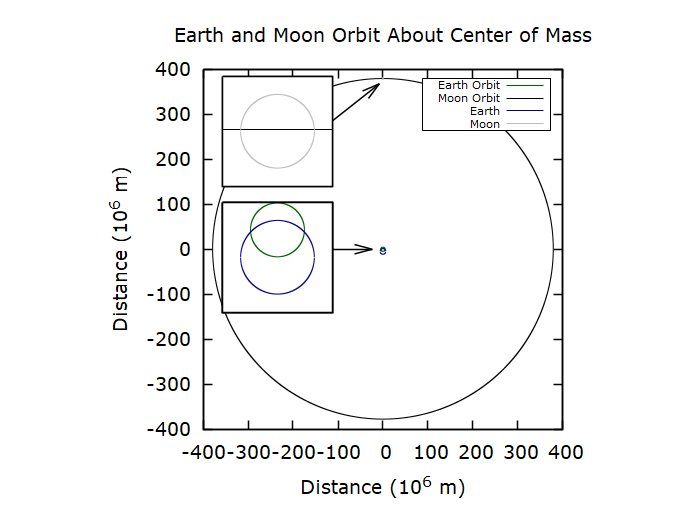
\includegraphics[scale=0.3]{em.png}
  		\caption{The orbital trajectories of the Earth and the Moon in the barycentric frame. assuming circular orbits. The Earth and the moon are drawn to scale here. Notice how the center of mas (the origin) is inside the Earth as we expect.}
  		\label{gr:earthmoon}
 	\end{center}
\end{figure}

\begin{figure}[htbp]
  	\begin{center}
 		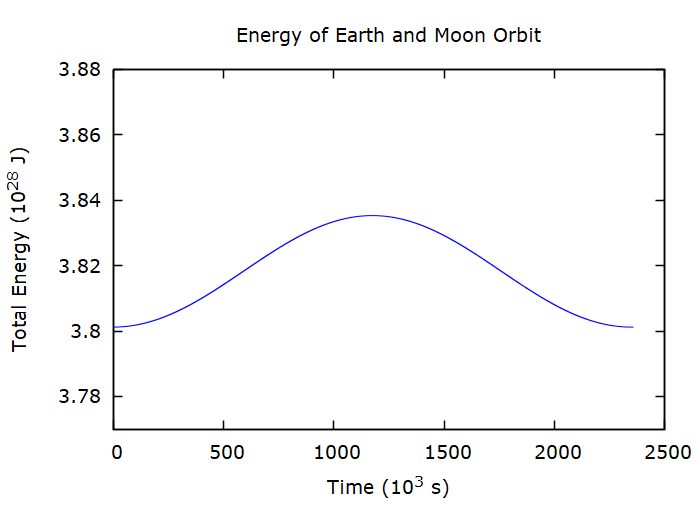
\includegraphics[scale=0.3]{orbit_energy.png}
  		\caption{The total energy of Earth and the moon in the barycentric frame. The energy is conserved to about 1\% using a time step of $dt = \SI{0.1}{\s}$.}
  		\label{gr:energy}
 	\end{center}
\end{figure}

\begin{figure}[htbp]
  	\begin{center}
 		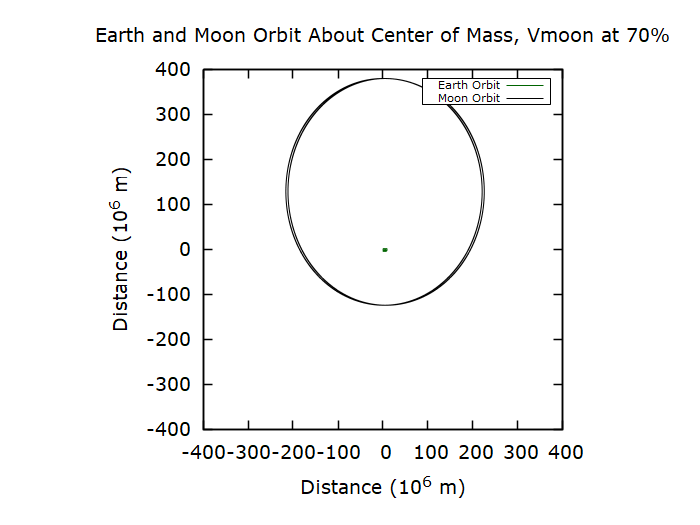
\includegraphics[scale=0.3]{emmoon70.png}
 		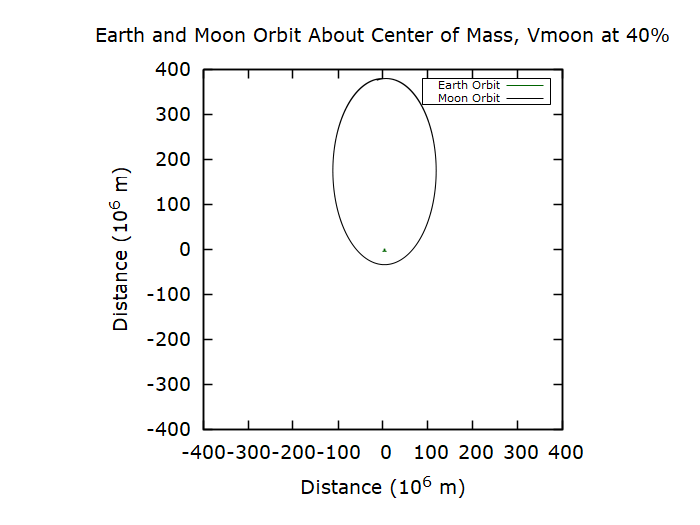
\includegraphics[scale=0.3]{emmoon40.png}
 		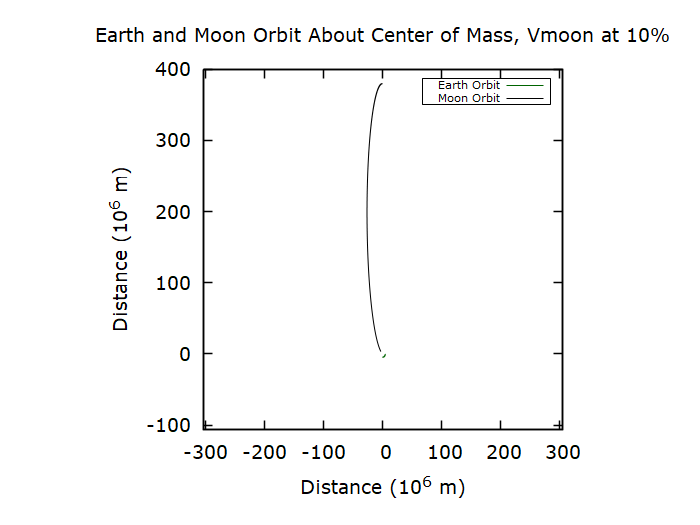
\includegraphics[scale=0.3]{emmoon10.png}
  		\caption{Here, we change the initial speed of the moon's orbit to 70\%, 40\%, and 10\% the original, necessary speed for a circular orbit. Clearly, lowering the kinetic energy of the moon results in a more elliptical orbit, until eventually there isn't enough energy to make it around the Earth and the moon just falls into it.}
  		\label{gr:slowmoon}
 	\end{center}
\end{figure}

\begin{figure}[htbp]
  	\begin{center}
 		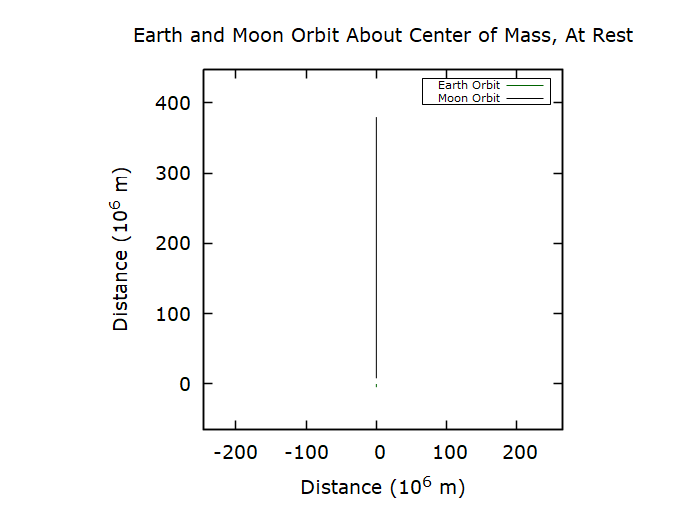
\includegraphics[scale=0.3]{emfall.png}
 		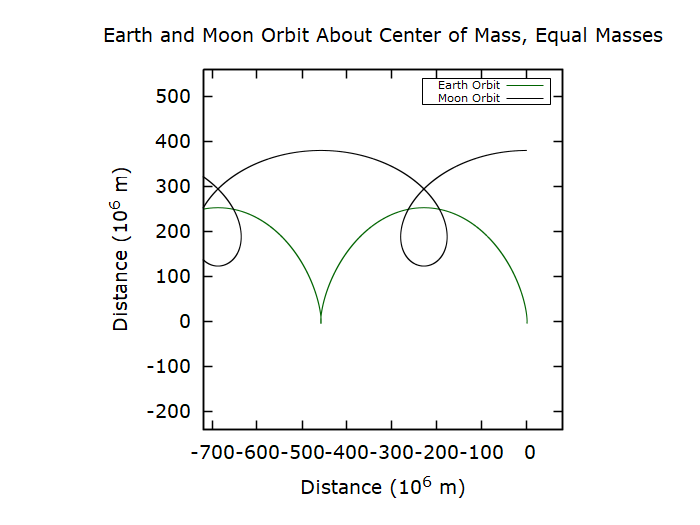
\includegraphics[scale=0.3]{emmass.png}
  		\caption{A couple of test demonstrations on how the orbits of the Earth and Moon change with different parameters. The plot above shows the Earth and moon falling into each other (zero intial velocity). The bottom plot shows the orbits for the Earth and moon having equal masses.}
  		\label{gr:test}
 	\end{center}
\end{figure}

\begin{figure}[htbp]
  	\begin{center}
 		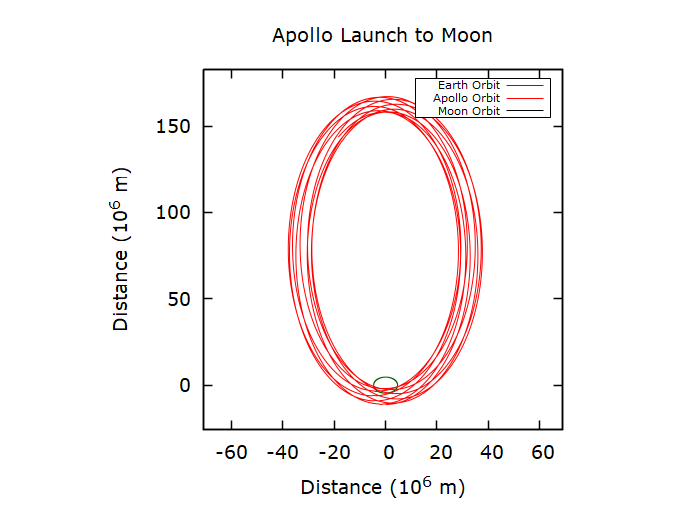
\includegraphics[scale=0.3]{1.png}
  		\caption{A low velocity launch at $\SI{2000}{\m\per\s}$, bringing Apollo to larger orbit than the parked orbit, but not enough energy to reach the moon.}
  		\label{gr:smalllaunch}
 	\end{center}
\end{figure}

\begin{figure}[htbp]
  	\begin{center}
 		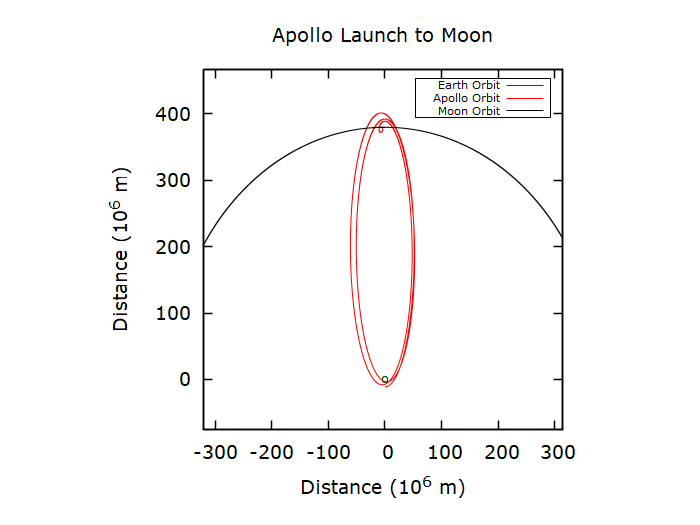
\includegraphics[scale=0.3]{launch_closest_try.png}
 		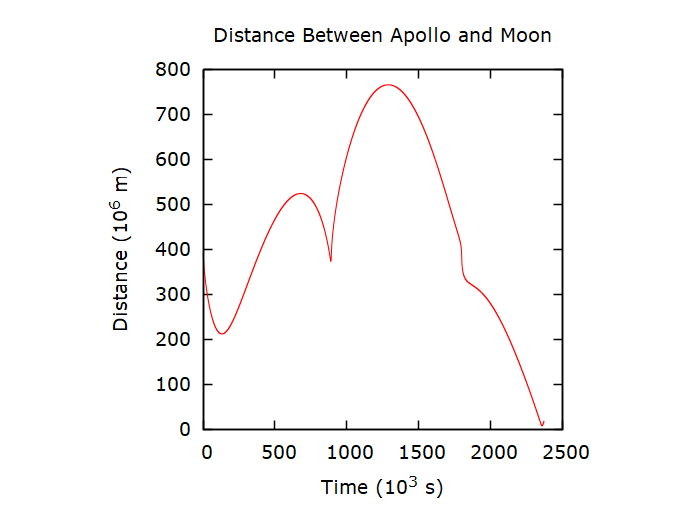
\includegraphics[scale=0.3]{dist.png}
  		\caption{Another trajectory to reach the moon. This time, Apollo began on the opposite side of the Earth from the moon. The initial launch parameters were $a = \SI{0}{\degree}$ above the x-axis and $v = \SI{3125}{m\s}$. Here, Apollo was able to reach an orbit that extended out to the moon and orbited three times during the moon's orbit before meeting the moon at the end.}
  		\label{gr:close}
 	\end{center}
\end{figure}

\begin{figure}[htbp]
  	\begin{center}
 		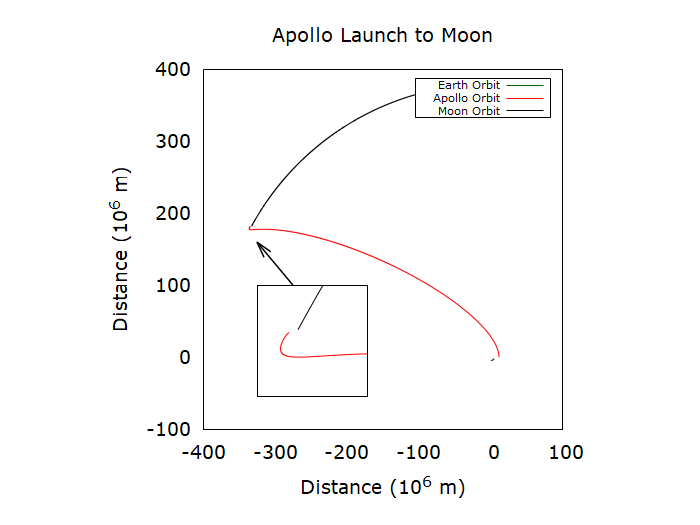
\includegraphics[scale=0.3]{hit.png}
 		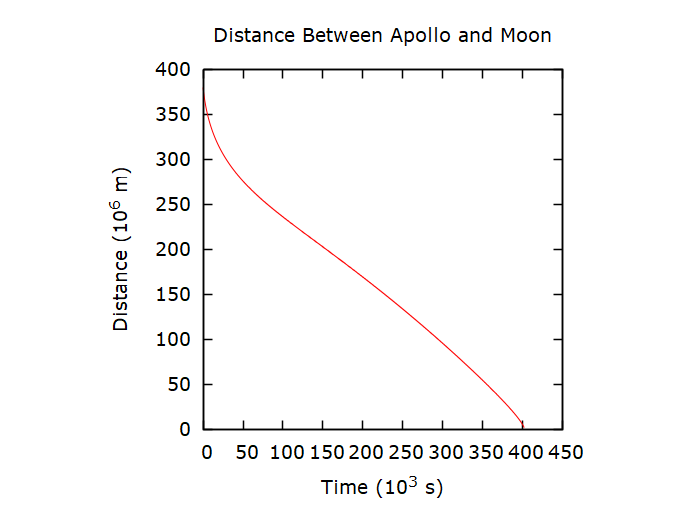
\includegraphics[scale=0.3]{disthit.png}
  		\caption{A successful launch to hitting the moon. The initial parameters were $a = \SI{13}{\degree}$ to the right of the y-axis and $v = \SI{160}{\m\per\s}$. These parameters obtained a trajectory with around the shortest time of about $\SI{4}{\day}$, meeting the moon before reaching the apogee. Apollo had slowed to a velocity of about $\SI{130}{\m\per\s}$ before being accelerated by the moon's gravity.}
  		\label{gr:hit}
 	\end{center}
\end{figure}

\begin{figure}[htbp]
  	\begin{center}
 		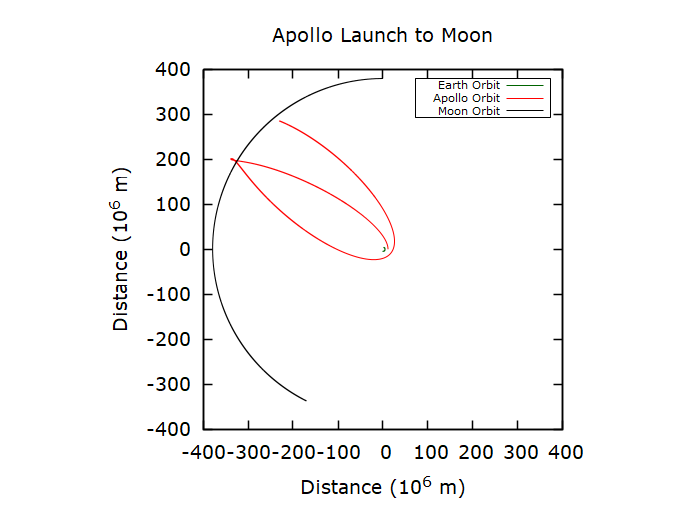
\includegraphics[scale=0.3]{back.png}
 		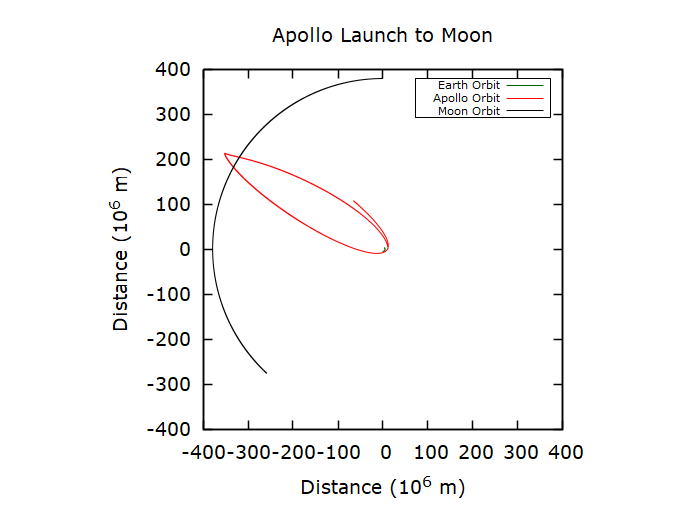
\includegraphics[scale=0.3]{back2.png}
  		\caption{The best solutions found to bring Apollo back to Earth using the moon's gravitational influence. The above plot used $a = \SI{40}{\degree}$ to the right of the y-axis, and $v = \SI{210}{\m\per\s}$. The plot below, which returned to Earth much closer, used $a = \SI{35}{\degree}$ to the right of the y-axis, and $v = \SI{207}{\m\per\s}$.}
  		\label{gr:back}
 	\end{center}
\end{figure}

\section{Discussion and Analysis}

\subsection{Earth-Moon System}
We start by simulating the Earth-Moon system, with our assumptions that simplified it. Initially, we set the bodies to be aligned on the y-axis with the moon on the +y side of the barycenter, the origin. We use the convention of counterclockwise motion, imparting a velocity according to Equation \ref{eq:orbvel} in the +x direction for Earth and in the -x direction for the moon. Figure \ref{gr:earthmoon} shows the path of the two bodies after one orbit of $T = \SI{27.321662}{\day}$. As we expect, the barycenter is within Earth's radius, but it is not exactly at the center of Earth.

The energy of the system through one orbit is shown in Figure \ref{gr:energy}. It appears to be oscillatory, and fluctuates between $\SI{3.8e28}{\joule}$ - $\SI{3.84e28}{\joule}$, conserving energy to about 1\% for a step size of $dt = \SI{0.1}{\s}$. 

Next, we examine some consequences of differing parameters of the Earth-Moon system. In Figure \ref{gr:slowmoon}, we change the initial velocity of the moon to a certain percentage of the original. One may expect at first to see the moon spiral into the Earth, but what actually happens is that the orbit becomes more and more elliptical. Eventually, the moon doesn't have enough energy to orbit the Earth and instead falls into it. 

In Figure \ref{gr:test}, we put the velocities to zero and let the bodies fall into each other. As we expected, the moon falls the greater distance and in fact, they both fall exactly into the center of mass (the origin). The total time elapsed was $\SI{4.82}{\day}$. This is the expected time for the moon to fall into the Earth, resulting from Kepler's third law \cite{phys}. Furthermore, we set the masses of the bodies to be equal and found that  the initial velocities (dominated by the moon) now pull the system to the side during the orbit. Notice now that they orbit a focal point that is equidistant to both bodies, as one should expect for equal mass objects.

\subsection{Apollo: Launch to the Moon}
We are now ready to introduce the Apollo spacecraft into our system. To choose the launch velocity $u$ and launch angle $a$, I used trial and error, with adjustments based on physical sense after viewing the resulting trajectories. 

At first, we let the spacecraft start below Earth (relative to the barycenter). Originally, I had assumed that since the Earth's velocity and Apollo's initial velocity added fully to the speed of Apollo, that we would not need much additional launch speed to get the spacecraft away from Earth. Instead, we found that an initial position like that required high velocities, three orders of magnitude high. Figure \ref{gr:smalllaunch} shows the resulting orbit of Apollo at $\SI{2000}{\m\per\s}$, and still not close to the orbital distance of the moon. An initial launch speed of $u = \SI{3125}{\m\per\s}$ was needed to reach the moon's orbit, and after one period of the moon's orbit, the two reached each other. This is shown in Figure \ref{gr:close}, as well as the distance between Apollo and the moon through time.

At such high velocities, there was no way to get a soft interaction with the moon. So instead, we try starting the spacecraft on the right side of Earth (again with respect to the barycenter). The required launch velocity to leave the Earth was much lower at this position. In Figure \ref{gr:hit}, we impart an initial velocity of $u = \SI{160}{\m\per\s}$ at an angle of $a = \SI{13}{\degree}$ to the right of the +y-axis. Apollo hit the moon in a "short" amount of time, making contact before reaching apogee. But the spacecraft had only slowed to about $\SI{130}{\m\per\s}$ by then, which was 10x larger than a steady orbital velocity around the moon below $\SI{500}{\km}$. 

Adjustments to that hit to find a working trajectory for orbiting the moon were not successful, but we did find trajectories that looped back, due to the moon's influence, towards Earth at low altitudes. Some of these resulting trajectories are shown in Figure \ref{gr:back}. The lower plot shows the closest approach back to Earth. This is a trajectory that would have been needed to bring the Apollo 13 astronauts back to Earth after launch. 

\section{Conclusions}
The efforts needed to send a spacecraft to the moon are incredible. The subtle changes in initial launch speeds and angles give dramatically different trajectories. This is why it is important to be so precise in these calculations. It is very impressive how the Apollo team has done to succeed in getting mankind to the moon.

Shown in this report are a handful of relatively successful results out of hours of trial and error in choosing the correct initial launch speed and angle. I can conclude that reaching the moon is indeed a difficult task. And this is only a simplified version of the true problem! To get a true depiction of the efforts needed, we need to incorporate features such as the eccentricity of the moon's orbit, the launch of the rocket as a function of time through Earth's atmosphere, etc. Luckily, we have computers that handle such massive calculations. It is then our jobs to implement the correct physics of the problem in our code. But still, great rigor and care is needed in that implementation, especially when the lives of others are at risk.

\section*{Acknowledgments}
\setlength{\parindent}{0cm}

\bibliographystyle{aipauth4-1}
\bibliography{bib10}



\end{document}